\newpage
\begin{Pro}
Para los siguientes DFA, obten el DFA minimo. 
\end{Pro}

Primero iniciamos con dos grupos, los estados de aceptacion y los estados que no son de aceptacion.

\begin{center}
\begin{align*}
    G_1 &= \{q_0\} && \text{Finales} \\
    G_2 &= \{q_1, q_2, q_3, q_4\} && \text{No finales}
\end{align*}
\end{center}

Como $G_1$ tiene un solo estado, es consistente y seguimos. 
Ahora revisamos el grupo de mayor consistencia en $G_2$. 


\begin{center}
\begin{tabular} {|c|c|c|}
    \hline
    $G_2$ & $a$ & $b$ \\ 
    \hline
    $q_1$ & $q_2 \in G_2$ & $\emptyset$ \\
    $q_2$ & $q_3 \in G_2$ & $\emptyset$ \\
    $q_3$ & $q_4 \in G_2$ & $q_0 \in G_1$ \\
    $q_4$ & $q_3 \in G_2$ & $q_0 \in G_1$ \\
    \hline
\end{tabular}
\end{center}

Dividimos $G_2$ en dos grupos nuevos, $G_2 = \{q_1, q_2\}$ y $G_3 = \{q_3, q_4\}$.

\begin{center}
\begin{tabular} {|c|c|c|}
    \hline
    $G_2$ & $a$ & $b$ \\ 
    \hline
    $q_1$ & $q_2 \in G_2$ & $\emptyset$ \\
    $q_2$ & $q_3 \in G_3$ & $\emptyset$ \\
    \hline
\end{tabular}
\end{center}

Vemos que $G_2$  no es consistente así que lo volvemos a dividir en $G_2 = \{q_1\}$ y $G_4 = \{q_2\}$.

\begin{center}
\begin{tabular} {|c|c|c|}
    \hline
    $G_3$ & $a$ & $b$ \\ 
    \hline
    $q_3$ & $q_4 \in G_3$ & $q_0 \in G_1$ \\
    $q_4$ & $q_3 \in G_3$ & $q_0 \in G_1$ \\
    \hline
\end{tabular}
\end{center}

Este grupo es consistente, por lo que ya no se puede dividir mas. Entonces los grupos finales son:

\begin{center}
\begin{align*}
    G_1 &= \{q_0\} && \text{Finales} \\
    G_2 &= \{q_1\} && \text{No finales} \\
    G_3 &= \{q_3, q_4\} && \text{No finales} \\
    G_4 &= \{q_2\} && \text{No finales}
\end{align*}
\end{center}

El DFA mínimo es:

\begin{center}
\begin{tabular} {|c|c|c|}
    \hline
    Estado    & $a$ & $b$ \\
    \hline
    $G_1$ & $q_1 \in G_2$ & $q_2 \in G_4$ \\ 
    $G_2$ & $q_2 \in G_4$ & $\emptyset$ \\
    $G_4$ & $q_3 \in G_3$ & $\emptyset$ \\
    $G_3$ & $G_3$ & $q_0 \in G_1$ \\
    \hline
\end{tabular}
\end{center}


\begin{figure}[h!]
        \centering
        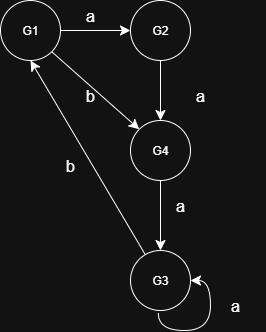
\includegraphics[width=0.4\textwidth]{images/ejercicio6a.png}
        \caption{DFA mínimo, ejercicio 6a}
\end{figure}
